%%%%%%%%                        01 - Motivace                       %%%%%%%%
%---------------------------------------------------------------------------
% Vážení posluchači, já bych Vám chtěl říct něco o své bakalářské práci na 
% téma Řešení futoshiki pomocí automatů.

%%%%%%%%                       02 - Cíle práce                      %%%%%%%%
%---------------------------------------------------------------------------
% Mým úkolem bylo navrhnout automat a na základě něho udělat implementaci, 
% která bude schopna řešit libovolnou mřížku Futoshiki. Dále jsem měl ukázat, 
% zda se pro řešení Futoshiki hodí dvojdimenzionální automaty.
\begin{frame}
  \frametitle{Cíl práce}
  \center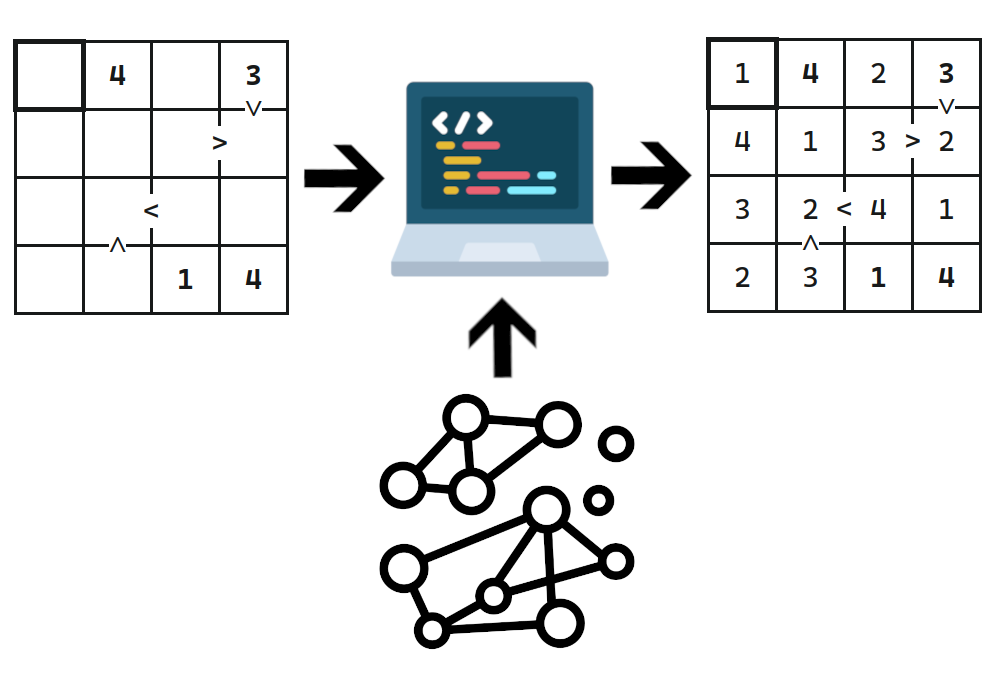
\includegraphics[width=\textwidth]{img/goal.png}
\end{frame}

%%%%%%%%                  03 - Informace o řešení                   %%%%%%%%
%---------------------------------------------------------------------------
% Co ale vlastně Futoshiki je? Je to logická hra, která se hraje na čtvercové
% mřížce o libovolné velikosti. Zpočátku mřížka obsahuje nějaká čísla a 
% popřípadě nerovnosti. Cílem je poté doplnit do mřížky čísla tak, aby byla 
% splněna dvě pravidla. První pravidlo je, že každý řádek i sloupec musí 
% obsahovat čísla od 1 do velikosti mřížky. Z toho vyplývá, že každé pole musí 
% mít v řádku i sloupci unikátní hodnotu. Druhé pravidlo říká, že musí platit 
% nerovnosti mezi čísly v mřížce.
\begin{frame}
  \frametitle{Co je futoshiki?}
  \centering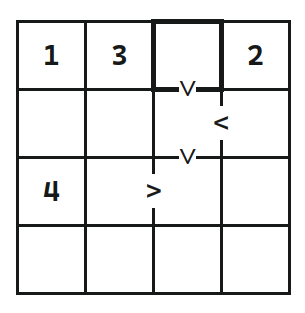
\includegraphics[width=0.4\textwidth]{img/futoshiki.png}
  \begin{enumerate}
    \item Každý sloupec a řádek čísla od \(1\) do \(n\)
    \item Platné nerovnosti
  \end{enumerate}
\end{frame}

% Jaké algoritmy lze tedy k řešení Futoshiki využít? Nejjednodušší možností
% je algoritmus Backtracking. Ten zkouší všechny možné kombinace, dokud 
% nenalezne řešení. Dále jsou tu algoritmy Forward Checking a Arc Consistency
% #3, které snižují počet kombinací, které je nutné vyzkoušet. Oba algoritmy
% si pro každé pole v mřížce uchovávají množinu možných čísel, kterou v
% průběhu běhu algoritmu upravují a eliminují tak neplatné kombinace.
% Forward Checking upravuje domény pouze přímo ovlivněných polí, tedy
% při zápisu hodnoty do žlutého pole se upraví pouze domény polí, která jsou
% zvýrazněna tyrkysově. Arc Consistency #3 potom upravuje domény všech 
% ovlivněných polí, v ukázce tedy i zelená pole.
\begin{frame}
  \frametitle{Algoritmy pro řešení}
  \begin{columns}
    \column{0.6\textwidth}
      \centering
      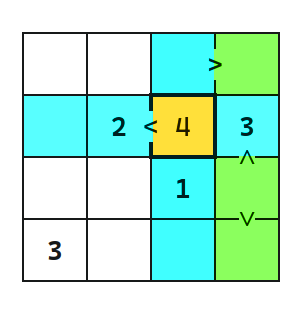
\includegraphics[width=1\textwidth]{img/futoshiki-relation.png}
    \column{0.4\textwidth}
      \begin{itemize}
        \item Backtracking
        \item Forward Checking
        \item Arc Consistency \#3
      \end{itemize}
    \end{columns}
\end{frame}

% Pro řešení Futoshiki jsem navrhl dvoudimenzionální skákající automat. Proč
% ale dvoudimenzionální? Futoshiki je hra, která se hraje na čtvercové mřížce,
% takže je pro člověka přirozené ji vnímat jako dvoudimenzionální. Dalším 
% důvodem je ale i usnadnění pravidel přechodů automatu. V případě, že by
% byla mřížka řešená jako jednodimenzionální, zvýšil by se počet stavů a
% například vyhodnocení nerovností by bylo složitější.
% Dvoudimenzionální skákající automat umožňuje pohyb ve čtyřech směrech, tedy
% nahoru, dolů, doleva a doprava. Navíc dovoluje i skoky, které umožňují 
% například skok na pole s nejmenší doménou, což zjednodušuje samotné řešení.
\begin{frame}
  \frametitle{Dvoudimenzionální skákající automat}

  \begin{columns}
    \column{0.6\textwidth}
    Sedmice \((Q, \Sigma, \Delta, R_1, R_2, s, F)\), kde:
    \begin{itemize}
        \item \(Q\) je konečná množina stavů.
        \item \(\Sigma\) je konečná množina vstupních symbolů.
        \item \(\Delta\) je množina povolených směrů.
        \item \(R_1\) je relace z \((Q \times \Sigma)\) do \((Q \times \Delta)\).
        \item \(R_2\) je relace z \(Q\) do \((Q \times \Sigma)\).
        \item \(s \in Q\) je počáteční stav.
        \item \(F \subseteq Q\) je množina konečných stavů.
    \end{itemize}

    \column{0.4\textwidth}
    \centering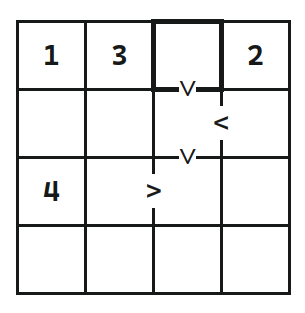
\includegraphics[width=1\textwidth]{img/futoshiki.png}
  \end{columns}
  \vspace{1.5em}
  \centering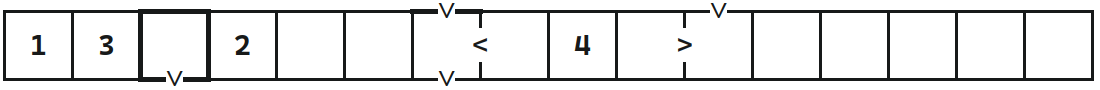
\includegraphics[width=1\textwidth]{img/1d-futoshiki.png}
\end{frame}


%%%%%%%%                    04 - Výsledky práce                     %%%%%%%%
%---------------------------------------------------------------------------
% Výsledná práce obsahuje jak návrh automatu, tak i pravidla pro řešení
% pomocí algoritmu Backtracking a Forward Checking. Dále jsem vytvořil 
% aplikaci s terminálovým rozhraním, která umožňuje uživateli vytvořit mřížku,
% nechat si vygenerovat náhodnou mřížku, složit mřížku a případně využít
% implementovaných algoritmů pro automatické řešení mřížky. Algoritmy, které
% využívají domény, jsou implementovány pro dva různé typy domén - pomocí
% hašovacích množin a pomocí bitmap. 
% Algoritmus Arc Consistency #3 pouze upravuje domény polí a dále neřeší 
% samotné vyřešení mřížky. Implementoval jsem proto dvě varianty řešení 
% - první varianta vygeneruje domény pomocí Arc Consistency #3 a poté využije
% Backtracking pro vyřešení mřížky. Druhá varianta je obdoba algoritmu 
% Forward Checking, jen se domény upravují pomocí Arc Consistency #3.
\begin{frame}
  \frametitle{Výsledky práce}

  \centering
  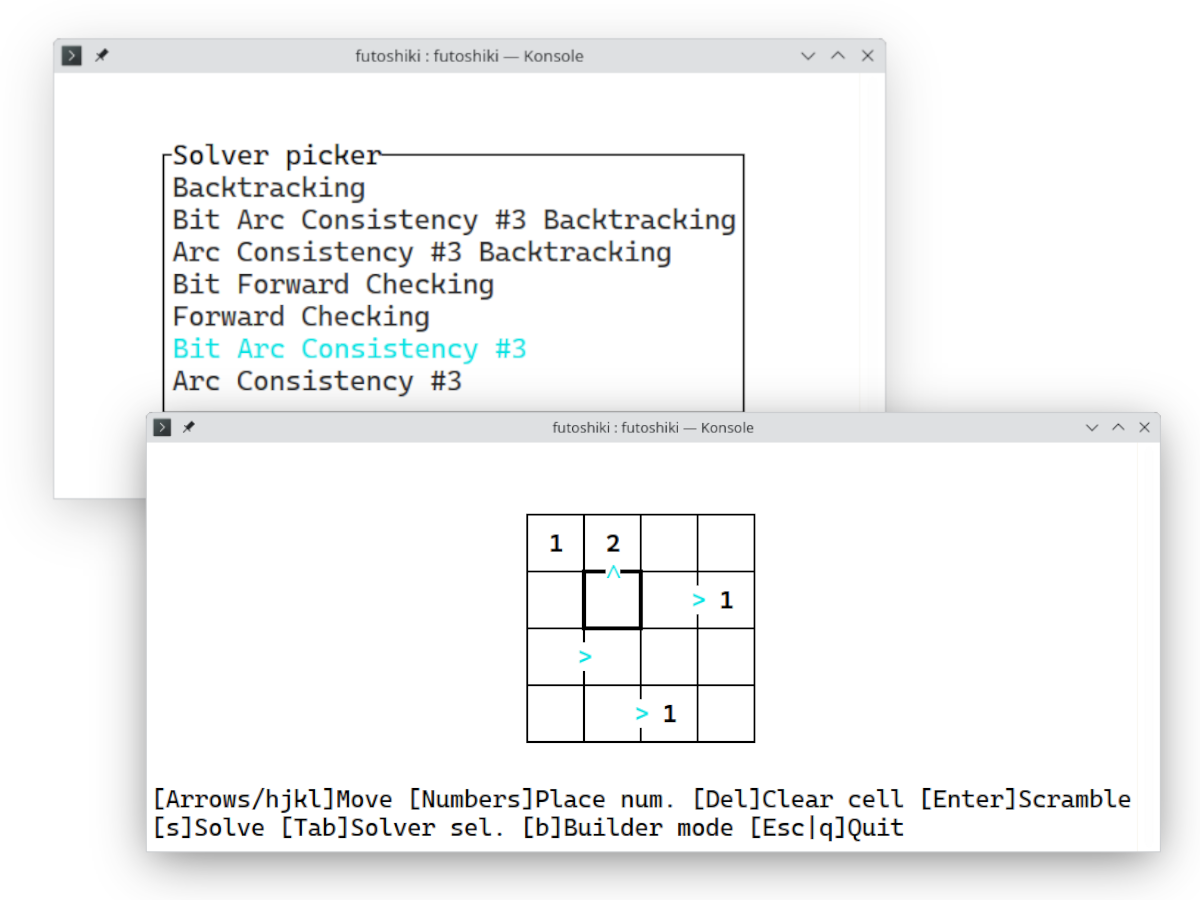
\includegraphics[width=1\textwidth]{img/implementation.png}
\end{frame}

% Implementace také obsahuje testy a benchmark. Benchmark porovnává časovou
% náročnost jednotlivých algoritmů na různých velikostech mřížek. Na obrázku
% vidíte výsledky benchmarku, který porovnává algoritmy na mřížkách od
% velikosti 4x4 do velikosti 10x10.
\begin{frame}
  \frametitle{Výsledky práce}

  \centering
  
\includegraphics[width=0.9\textwidth]{img/benchmark.png}
\end{frame}

% Navíc je možné porovnat i časovou náročnost operací nad různými typy domén 
% a využití paměti jednotlivých domén. Testování proběhlo na třech různých
% typech domén - pomocí hašovacích množin, bitmap a pomocí vektorů.
\begin{frame}
  \frametitle{Výsledky práce}

  \centering
  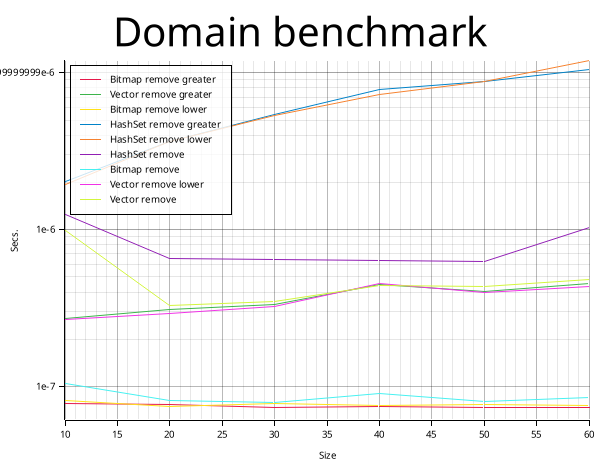
\includegraphics[width=0.9\textwidth]{img/domains_benchmark.png}
\end{frame}

%%%%%%%%                      05 - Poděkování                       %%%%%%%%
%---------------------------------------------------------------------------
% To by z mé strany bylo vše a já vám děkuji za pozornost.
\begin{frame}
  \frametitle{Děkuji za pozornost!}
  \center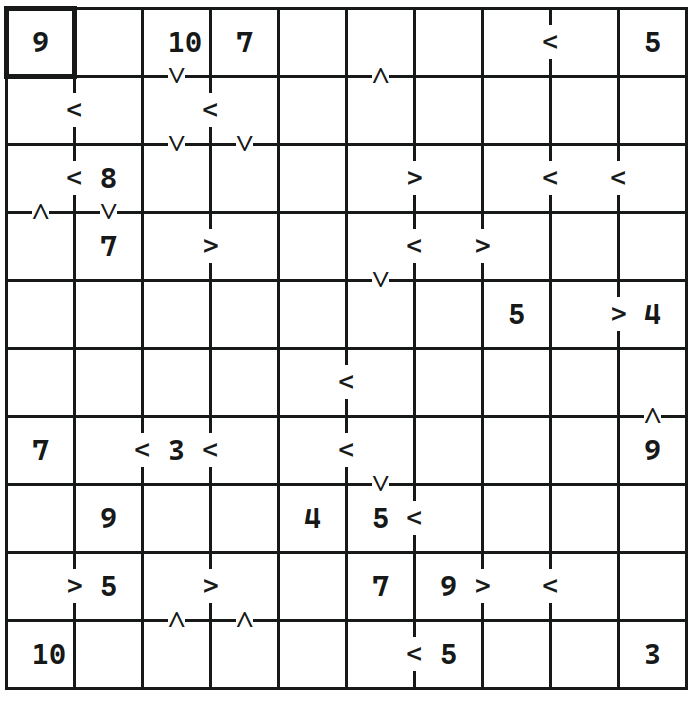
\includegraphics[width=0.7\textwidth]{img/futoshiki-large.png}
\end{frame}
